\subsection{Charakterystyka}

	\begin{enumerate}
		\item{\textbf{Zakup towarów}} - koszt zakupu towaru przez klientów.
		
		\item{\textbf{Ubezpieczenia rzeczowe}} - są to niezbędne ubezpieczenia sprzętu komputerowego.
		
		\item{\textbf{Koszty administracyjne }}
			\begin{enumerate}
				
				\item{\textbf{Reklama}} - koszty związane z pozycjonowaniem strony, reklamie internetowej, kolportażu ulotek, które pozwolą na promowanie mojego sklepu.
				
					\begin{enumerate}
					
						\item{\textbf{Kolportaż ulotek}} - koszty związane z kupnem i drukowaniem ulotek 
		
						\item{\textbf{Bilbord}} - koszty związane z wynajęciem bilbordu
					
					\end{enumerate}
					
				\item{\textbf{Wynagrodzenie pracowników}} - koszt wynikający z planowanego zatrudnienia w drugim i trzecim roku prowadzenia działalności.
			
				\item{\textbf{Narzuty wynagrodzenia}} - są to wszystkie obowiązkowe obciążenia narzucone na pracodawcę z tytułu zatrudnienia pracowników. Są to: składki z tytułu ubezpieczenie społecznego, składki na Fundusz Pracy i Fundusz Gwarantowanych Świadczeń Pracowniczych, odpisy na Zakładowy Fundusz Świadczeń Socjalnych.
			
				\item{\textbf{Energia}} - na koszty utrzymania systemu składać się będą koszty prądu.
					\begin{enumerate}
						
						\item{\textbf{Prąd}} - koszty powstałe na skutek wykorzystania systemu komputerowego \label{prad}
						
						\item{\textbf{Ogrzewanie}} - koszty powstałe na skutek ogrzewania obiektu 
						
					\end{enumerate}
					
				\item{\textbf{Usługi obce}} - zostały tu ujęte usługi księgowe, których szacowany koszt miesięczny wynosi 200 zł.
			
				\item{\textbf{Podatki lokalne}} - podatek od powierzchni, na której będę prowadzić działalności.

				\item{\textbf{inne koszty}} składka na ubezpieczenie  społeczne  właściciela.
			
				\item{\textbf{Koszty telekomunikacyjne}} - Do kosztów telekomunikacyjnych należy wliczyć koszt utrzymania połączenia internetowego, ze względu na konieczność utrzymywania dwóch adresów IP co wynika wprost z rfc1035, określającego parametry łączą dla przechowywania domeny, daje 110zł/m-c. Dla łączą o parametrach 2 x 100/100Mbps. Do kosztów tych należy doliczyć jeszcze koszt dwóch numerów w Polsce i Kanadzie z nielimitowanym planem taryfowym 70zł/m-c przy wykorzystaniu technologii VOIP (Voice Over IP).
		
				%\item Amortyzacja - koszt związany ze stopniowym zużywaniem się środków trwałych i wartości niematerialnych i prawnych. Dokonałam jednorazowej amortyzacji na kwotę 5667 zł.- pomoc de minimis. Dotyczy ona zakupu procesorów serwerowych.
			\end{enumerate}
				
	\end{enumerate}		

			
		\paragraph{Koszty prądu-uzasadnienie \cref{prad}}		
			
			
	\par Koszty prądu można wyliczyć posługując się danymi ze specyfikacji technicznej sprzętu komputerowego. Zużycie prądu w watach przedstawia poniższa lista:
	
			\begin{itemize}
				\item{\textbf{Procesor}} - 85W
					
				\item{\textbf{Płyta główna}} - 70W
					
				\item{\textbf{Pamięć operacyjna}} - 4W
					
				\item{\textbf{Dysk twardy HDD}} - 8W
					
				\item{\textbf{Dysk twardy SSD}} - 3W
					
				\item{\textbf{Karta graficzna}} - 15W
			\end{itemize}

			\par Co po przemnożeniu przez ilość elementów określonych w wycenie daje:
						
			\begin{itemize}
				\item{\textbf{Procesor}} - 255W
					
				\item{\textbf{Płyta główna}} - 210W
					
				\item{\textbf{Pamięć operacyjna}} - 24W
					
				\item{\textbf{Dysk twardy HDD}} - 32W
					
				\item{\textbf{Dysk twardy SSD}} - 9W
					
				\item{\textbf{Karta graficzna}} - 45W
			\end{itemize}
				
		\par Daje to sumaryczne zużycie prądu przez sprzęt komputerowy 575W. Należy wziąć tu jeszcze pod uwagę sprawność zasilacza, która dla wybranego modelu wynosi ok. 80\%. Znaczy to, że sprzęt komputerowy poprzez straty na zasilaczu będzie pobierał 20\% energii więcej co daje ok. 690W. Wliczając w to pobór prądu przez urządzenia takie jak: kasa fiskalna, router, drukarka, switch daje ok 800W. Biorąc pod uwagę pracę systemu 24 godziny na dobę przez cały rok daje zużycie energii na poziomie 7000 kWh rocznie. Do tych kosztów należy doliczyć jeszcze energię zużytą przez komputer na stanowisku pracowniczym pracujący 8 godzin dziennie przez 250 dni, (tyle bowiem średnio jest dni pracujących w roku) pobierający ok. 80W energii na godzinę. Daje to zużycie prądu rocznie na poziomie 160 kWh. Na tej podstawie można oszacować średnie roczne zużycie prądu 7150 kWh. Czyli w ujęciu miesięcznym 595 kWh, co biorąc pod uwagę średni koszt kWh prądu na Dolnym Śląsku ok. 0.55 zł/kWh daje szacunkowo 320zł/m-c. Zakładając 5\% niedoszacowanie wartości wychodzi ok 340zł/m-c. Odchylenie to wynika z szacowania poboru prądu dla urządzeń w stanie pracy bez obciążenia. Nie będzie to już w tym wypadku wartość znacząca, jednak warto o pamiętać o tym fakcie.
	
	
	\par Do kosztów  należy również doliczyć zakup niezbędnego zaopatrzenia biura. Dzielimy je na:
	
			\subsubsection{Zakupy jednorazowe}
					\begin{itemize}
						\item Niszczarka - urządzenie służące do niszczenia poufnych dokumentów, najczęściej wykorzystywane do zastosowań biurowych. 
						\item Szafka kartotekowa - mebel służący do przechowywania i segregowania dokumentów. 
						\item Półki na dokumenty - meble służące do przechowywania i składowania dokumentów. 
						\item Tablica magnetyczna - element biura służący do przypinania na niej ważnych informacji.
						\item Kalkulator - urządzenie służące do obliczania wartości matematycznych. 
					\end{itemize}	
						
			\subsubsection{Zakupy okresowe}
					\begin{itemize}
						\item Papier do drukarki - niezbędny do drukowania na nim dokumentów, faktur, umów itp..
						\item Tusz do pieczątki - niezbędny element pieczątki mający na celu uzupełnianie w niej braku tuszu. 
						\item Bloczek samoprzylepny - służy do zapisywania informacji i przyklejania do powierzchni  stałych np.tablicy magnetycznej. 
						\item Koperty - papierowe opakowania, przeznaczone do przesyłania w nich listów lub innych przesyłek pocztowych.
						\item Długopisy - narzędzie służące do zapisywania informacji na papierze. 
						\item Zakreślacze - służą do podkreślania ważnych informacji. 
						\item Segregatory na dokumenty - element biura mający na celu segregowanie dokumentów. 
						\item Teczki na dokumenty - przedmioty służące do przenoszenia; segregacji dokumentów. 
						\item Taśma bezbarwna - ma na celu łączenie elementów; sklejanie ich. 
						
					\end{itemize}	

					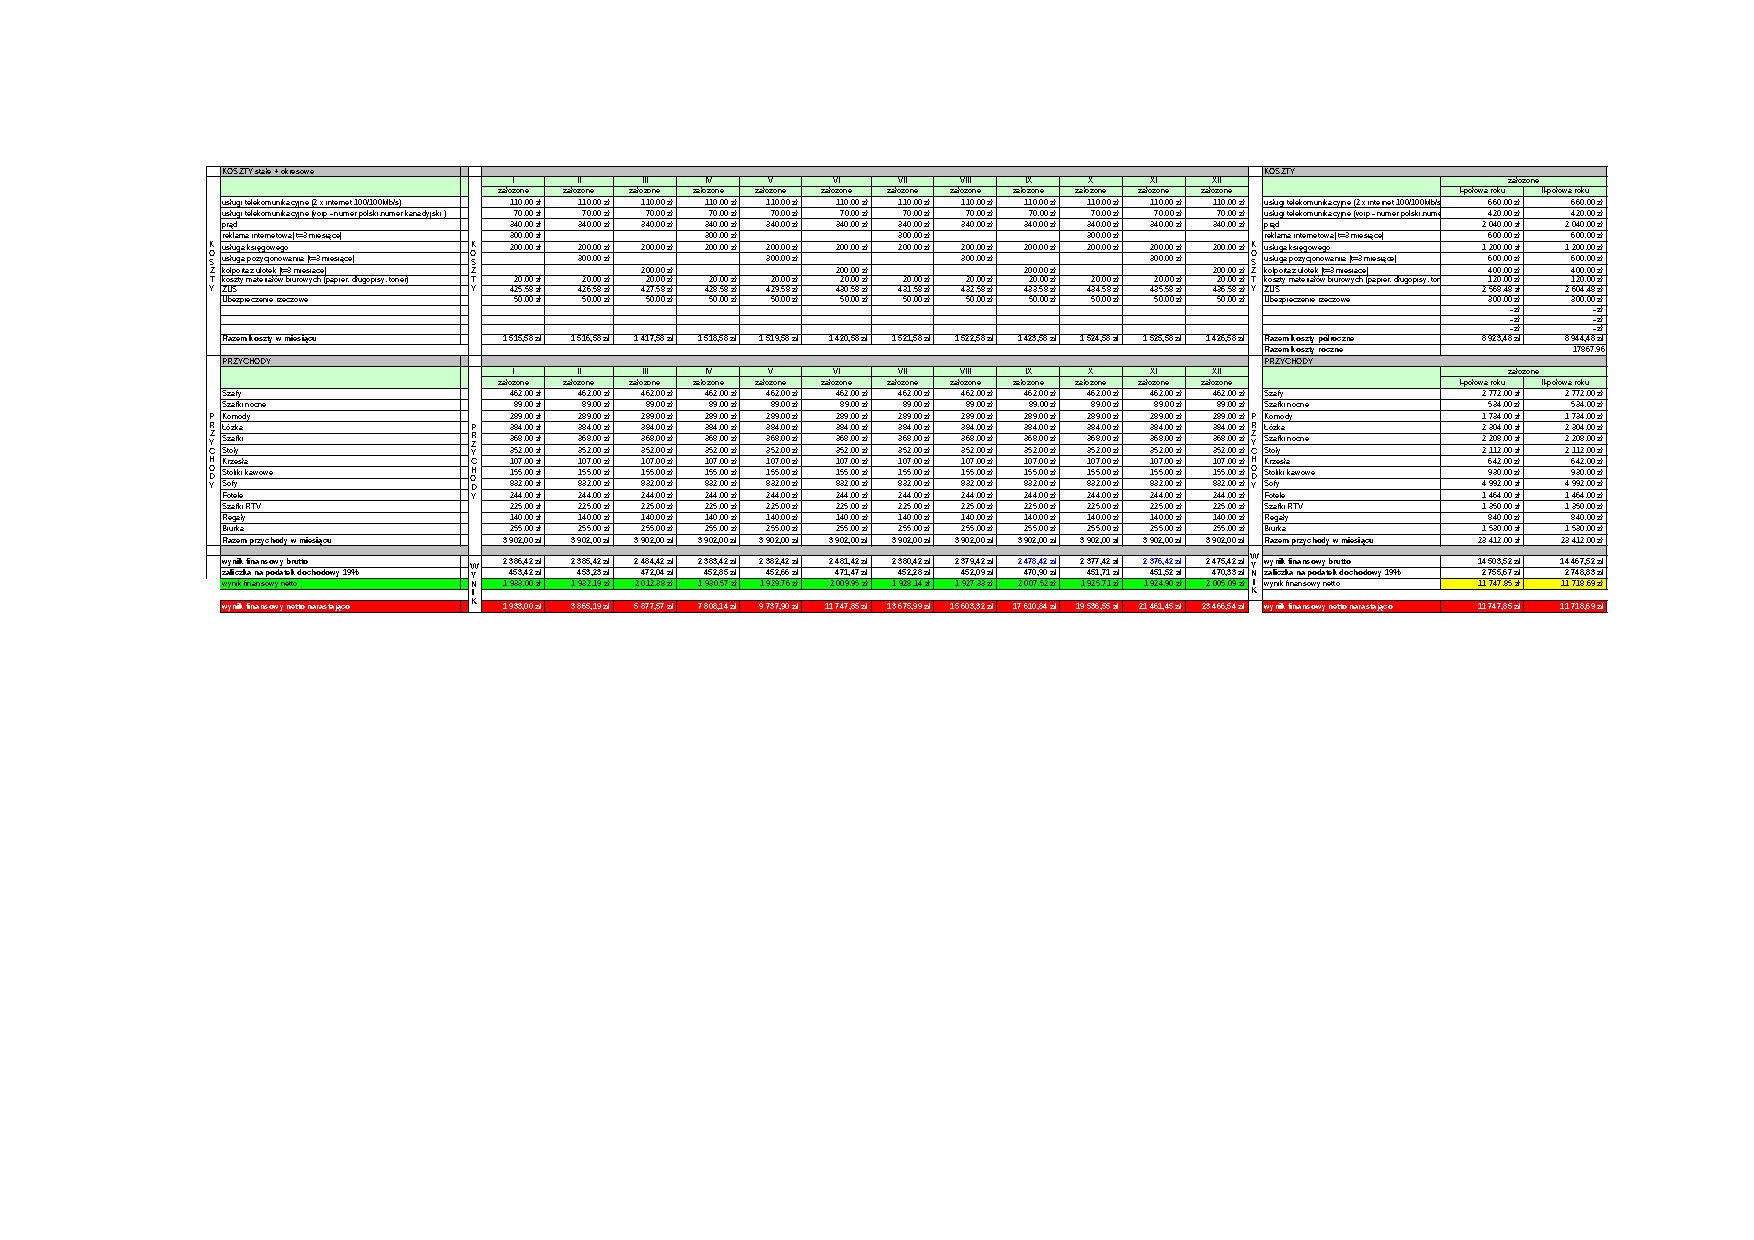
\includepdf[pages={1-},angle=270]{koszty.pdf}
